\section{Linux实现}
\subsection{Spin lock}
自旋锁是一种特别的锁机制,
使用自旋锁的进程无法获得锁时进入忙等待、重试直至成功,
而不是象~{\em semaphore}~机制那样睡眠等待唤醒。
Linux~自旋锁隐含着禁用内核抢占,
所以有进程在获得自旋锁之后睡眠几乎一定导致死锁。

自旋锁由于需要对位于内存中的锁变量进行``读--改--写''操作,
所以必须有硬件指令保证完成这一操作的原子性,
亦即自旋锁的最终实现是硬件相关的。
以下仅以Intel平台为例,
传统的自旋锁实现如下:
\inputclisting{src/spinlock.h}
              {traditional implementation of spin lock}{ospl}
注意dec是一条``读--改--写''指令,
Intel提供了lock指令锁住内存总线,
由lock修饰的指令执行结束之前其它CPU和DMA设备无法访问内存,
这正是spin lock在Intel平台得以实现的基础。
上锁算法思路是
\begin{enumerate}
  \item 将锁变量值(原子地)减1。
  \item 测试状态寄存器(EFLAGS)的符号位(SF),
        如果为0,
        说明之前的锁变量值为正,
        线程成功获得锁进入临界区代码。
        \verb|js 2f|的下一条指令位于调用者指令序列处,
        而\verb|LOCK_SUBSECTION_START|是内核专门定义一个 subsection 存放自旋部分代码,
        \verb|ld|会将自旋部分代码移至它处(即所谓{\em relocation})。
        \footnote{
        因为上锁操作大部分情况下成功,
        自旋代码不和其它指令混合可以防止指令缓存污染,
        由于自旋锁大量使用,
        微小的效率损失不容忽视。}
  \item 如果上锁失败,
        程序跳转进入自旋部分代码,
        自旋部分不断测试锁变量直至发现其值大于0,
        此时必须重复步骤1,
        下一个成功将锁变量减为0的线程获得锁。
\end{enumerate}

解锁操作仅需将锁变量值重置为1即可,
写操作自然是原子的。

传统自旋锁的实现最大问题是可能导致不公平,
自内核2.6.25始,
新的队列自旋锁被引入,
实现如下:
\inputclisting{src/ticket_spinlock.h}
              {ticket spin lock}{tspl}
算法思路是将锁变量分成两部分操作,
高16位为抢占位段(可理解为为该线程分配的票号),
即指示需要上锁的线程在队列中的位置;
低16位为准入位段(当前准许进入临界区的票号)。
更具体地说,
需要上锁的线程读入准入位,
将抢占位段加1,
之后开始忙等待直至察觉它的抢占位(代码中的\verb|inc|变量的高16位)%
和内存中锁变量的准入位段(不停地通过movb从内存中读入\verb|tmp|)%
一致时获得锁进入临界区。
代码中关键指令是\verb|xaddl|,
该指令完成将源/目标操作数交换并且将源/目的操作数的和写入目的操作数,
这一操作同样使用\verb|lock|前缀保证原子性。
解锁操作原子地将准入位段加1即可。

\subsection{读--写锁及seqlock}
spinlock并不区分对共享内存的访问类型,
一概地串行化,
但对共享内存区域的读访问之间并不需要同步,
于是读--写自旋锁被引入。
简而言之其思路为,
读--读访问不互斥,
但写--写和读--写访问仍然按自旋锁方式同步。
具体到代码,
实现思路为将32位锁变量分为两部分,
低24位(0--23)作为读者计数,
第24位为锁标志位(置1表示解锁,反之为上锁)。
锁变量初始化为0x01000000,
即0读者解锁状态;
读者上锁通过对锁变量原子地减1(亦即读者计数加一)%
如果发现符号位SF未置,
说明之前是解锁状态,
可以获得读锁进入临界区,
否则就spin直至成功。
解读锁仅需要对锁变量加一;
而写者上锁需要将锁变量减去0x01000000而后观察ZF标志,
即判断差是否为0,
是则获得写锁进入临界区,
否则忙等待直至成功。
解写锁即将锁变量加上0x01000000。
代码如下:

\inputclisting{src/rw_lock.h}
              {read-write spin lock}{rwspl}
其中上锁失败后调用的helper就是spin部分,
x86汇编代码如下:
\inputasmlisting{src/rwlock_failed.S}
              {read-write spin lock helpers}{rwlf}

读--写锁的一个问题是读和写操作没有优先级差别,
当需要尽快满足写操作时,
可以使用内核提供的seqlock。
在这种情况下,
写者获得锁的优先级高于读者,
当然写者仍然需要等待另一位写者结束解锁后才能进入临界区。
具体实现思路如下:
锁变量类型seqlock\_t有两个域,
其中一个为自旋锁用于写者间同步,
另外一个为初始值为0的整数用作写序列号,
写者获得自旋锁之后将序列号加一,
解锁时再加一,
于是当写者位于临界区内是,
写序列号为奇数,
否则为偶数。
读者在读共享数据之前之后都读取写序列号,
如果写序列号没有变化并且为偶数,
说明在读过程中数据没有被改动,
继续执行,
否则需要重新读取数据直至成功。
seqlock主要实现如下:
\inputclisting{src/seqlock.h}
              {seqlock}{seql}
读过程通常如下所示:
\inputclisting{src/seqlock_read.h}
              {read with seqlock mechanism}{rseql}
显而易见seqlock的一个缺点就是读者可能不得不反复读取无效的数据很多遍。

\subsection{原子类型变量}
在X86平台下,
以下场景的原子性值得留意:
\begin{itemize}
  \item 单次访问地址对齐({\it aligned})的内存对象是原子的
  \item 诸如inc、dec这类的读--改--写操作如果在读之后,写之前%
    没有其它CPU访问内存,
    该操作是原子的,
    也就是说读--改--写操作在单CPU系统中是原子的
  \item 带lock前缀的读--改--写操作是原子的
  \item 带rep前缀指令的多次迭代{\em 不是}原子的
\end{itemize}
程序员可以依据上述原则在汇编程序中控制对变量原子性,
但是编写C程序时不能对编译器生成代码做任何假设,
诸如i++这样的语句无法保证原子性,
于是原子类型变量(atomic\_t)被引入为了保护单个共享的整形变量。
原子类型定义及基本操作代码如下:
\inputclisting{src/atomic.h}
              {atomic type and operations}{at}
可以看出,
单单读写不需要特别的处理,
C的赋值语句就保证了原子性,
加减之类涉及读—改—写操作才需要汇编指令保证原子性。
值得一提的是atomic\_sub\_and\_test的实现,
sete指令结果依赖于ZF标志位,
而该标志位的设置和subl是一个原子操作,
有效性可以保证。

内核中大量使用一种技术——{\em 引用计数}{\em reference counting},
即资源使用者在使用前将计数加一({\em get}),
使用结束后减一({\em put}),
计数表明当前使用者数量,
当发现该计数为零的时候,
可以安全地将共享资源释放。
该计数使用方式大体有两类,
区别在于put的处理:
\begin{enumerate}
  \item {atomic\_dec\_and\_test}:
    这种方式见于内部逻辑使用一个计数进行同步,
    例如MCOpt的proc层通过threads计数来记录当前线程数,
    主线程创建时计数初始值设为1,
    之后每创建一个新线程,
    父线程调用get\_proc\_info,
    即atomic\_inc来增加threads计数,
    每个线程结束时调用put\_proc\_info,
    即atomic\_dec\_and\_test来减少计数同时(原子地)检查计数是否降到0,
    发现计数为零的那个线程就认为它是唯一存活的线程,
    可以安全地释放proc结构。
    不可能在计数降为0之后还有其它线程调用get,
    因为get{\em 只}在fork的时候调用,
    而fork肯定发生在exit之前,
    此时调用fork的线程本身还占用一个计数于是不可能有线程在那之前就观察到计数降为0的情况。
    所以使用此机制要保证一条原则:
    get/put配对,
    先后顺序必须保证。

  \item {atomic\_dec\_and\_lock}:
    这种方式见于内部逻辑和外部逻辑都使用该计数,
    但是外部逻辑另外需要一个锁来同步。
    一个例子是内核vfs的iput函数,
    它调用atomic\_dec\_and\_lock函数减少inode计数,
    如果计数为零,
    将计数降为零的线程原子地把全局inode\_lock也一同锁上,
    而后调用iput\_final把inode对象释放掉,
    释放过程包括把inode从一个链表上删除的操作。
    之所以要保证dec和lock两个操作的原子性是因为:
    可能有其它函数(外部逻辑)以``相反''的顺序进行上锁和增加计数,
    如ifind\_fast函数,
    它对inode\_lock上锁成功后遍历链表,
    当找到目标inode后,
    对其实行get操作,
    如果iput函数中的dec和lock不原子,
    调用iput的线程在将inode的计数减到0之后却没能抢到锁,
    而此时正持有该锁的线程执行lookup成功将该值加1以为从此可以放心使用,
    当执行iput的线程得到锁以后不重新检查计数就释放该inode,
    问题出现了。
\end{enumerate}
atomic\_dec\_and\_lock的实现比较有趣,
C内嵌汇编的代码如下:
\inputclisting{src/dec_and_lock.c}
              {Atomic Dec And Lock C code}{adalc}
其实现是硬件相关的,
高效的版本利用了Intel处理器提供的cmpxchg指令。
从反汇编出来的代码可以将代码思路看得更清楚:
\inputasmlisting{src/dec_and_lock.S}
                {Atomic Dec And Lock assembly code}{adala}
地址ffffffff801f6c64的指令将atomic变量值从内存读入esi寄存器,
地址ffffffff801f6c6b的指令将变量值减去一的结果存入eax寄存器%
(注意lea指令并不改变esi),
之后又被转移到rdi中。
关键指令是那条cmpxchg语句,
它比较rax和目的操作数(这里是rbx间接寻址的内存)的值,
如果相等,
将源操作数(这里是edi)中的值存入目的操作数中,
否则将目的操作数中的值读入rax,
重要的是整个过程原子地完成。
具体到这段代码就是:
如果atomic变量值从开始读入esi一直到执行cmpxchg期间没有被其它线程改动过,
edi中的值就会被写入atomic变量中,
orax也不会被改变,
即dec成功,
之后就跳转到调用spin\_lock;
如果ffffffff801f6c7b地址处的比较发现cmpxchg改变了rax的值,
意味着atomic变量在中途被改动了,
不能对atomic变量做任何修改,
只能将被其它线程改动后的新值读入esi,
跳回ffffffff801f6c66重新开始尝试dec操作。
\subsection{Semaphore}
(从略)
\subsection{Per-CPU 变量}
所有的锁算法都会引入大的开销,
所以最好的同步方案是在设计过程中想办法避免同步。
在某些场合下使用Per-CPU变量可以起到免同步的效果。
简而言之,
Per-CPU变量是一个数组,
数组元素和CPU一一对应,
在某个CPU上运行的线程只能访问该CPU对应的数组元素,
于是无须在运行于不同CPU的线程间同步对该变量的访问。
唯一需要防止的一种情况是内核抢占,
所以在访问Per-CPU变量时必须禁用内核抢占。
Per-CPU变量机制常用的几个接口是:
DEFINE\_PER\_CPU(type, name),
get\_cpu\_var(name),
和put\_cpu\_var(name),
其中put\_cpu\_var(name)仅仅是启用内核抢占,
并不使用其参数。

\subsection{RCU}
RCU({\em Read-copy update})%
被发明用于保护通过指针访问的共享数据。
尽管其某些接口使用了类似lock、unlock这样的名称,
当只有一个写者的时候RCU事实上是一种免锁方案,
亦即无全局共享的锁或计数存在,
多个写者之间仍然需要用自旋锁同步。
正确使用RCU的两个限制条件:
\begin{enumerate}
  \item RCU只用于通过指针访问的共享内存区域
  \item 位于RCU\,``临界区''内的代码不允许阻塞
\end{enumerate}

RCU机制也分为读者和写者,
读者``上锁''和``解锁''仅需要禁用和启用内核抢占即可;
写者则相对复杂一些,
它需要完成拷贝共享的数据结构到一个新分配的地址,
写入数据结束之后将共享数据的指针改为新地址,
由于指针赋值是原子的,
于是读者读取的数据来源不是旧指针指向的区域就是新指针指向的区域,
但一定是有效的。
保证数据有效性需要注意的是RCU必须使用内存屏障以%
保证对新内存区域的写和修改指针的先后顺序。
一般而言,
RCU在大量读操作极少数写操作的情况下是读--写锁的一个高效替代品。
在RCU引入之后,
如路由表维护、dcache以及System V IPC的部分的代码迅速采用此机制。
\inputclisting{src/rcu.h}
              {RCU's dereference and assign pointer}{rcu}

RCU实现中需要解决一个重要问题是修改指针之后,
旧指针指向的内存区域应该在{\em 适当}的时候被释放。
先说写者,
写者需要在修改指针之后注册一个回调函数以期在未来某个时候被调用释放内存,
事实上对指针的修改操作也可以放在回调函数中,
但这可能导致修改的可见性出现一定的延迟。
再说读者,
当CPU经过如下{\em quiescent state}(即该CPU处于可抢占状态)%
之前读者必须已经调用过rcu\_read\_unlock,
\begin{itemize}
  \item 进程切换(参看使用RCU的第二个限制条件)
  \item 开始进入用户空间运行
  \item 内核调度idle线程
\end{itemize}
当所有的CPU都进入quiescent state之后,
我们称一个{\em grace period}结束,
即所有的CPU都处于可抢占状态,
可以推断所有的读者已经``解锁'',
此后再有一个时钟中断来临,
RCU的垃圾回收器将调用写者注册的回调函数安全地释放掉旧指针指向的内存。
以下是几种RCU的使用案例:
\subsubsection{链表遍历、增加及删除}
在增加删除操作不常发生的情况下,RCU可以高效地同步链表操作。
内核2.6增加了使用RCU的链表操作接口,
如list\_add\_rcu、list\_del\_rcu等,
定义如下:
\inputclisting{src/list_rcu.h}
              {list protected by RCU}{listrcu}
几个值得注意的要点:
\begin{itemize}
\item list\_del\_rcu在删除完某个节点之后并不是把该节点的前后向指针都置为poison,
  因为该节点可能正在被某个读者用于遍历链表。
\item \_\_list\_add\_rcu函数中使用了写内存屏障,
  在%list\_for\_each\_entry\_rcu调用的
  rcu\_dereference宏中%
  使用了与之配对的数据依赖内存屏障,
  这一对内存屏障保证了如果读者通过访问某个节点的next或prev看见了新节点,
  那么在数据依赖屏障之后看见新节点的prev/next值必然是写屏障之前的值。
  在内核2.4中对协议链表的保护采用读--写锁。
\end{itemize}

一个较早开始使用RCU保护链表的例子是内核网络L3协议注册、注销、分派%
({\em dispatch})等部分的代码。
先看协议分派部分(读者)的代码:
\inputclisting{src/netif_rx.c}
              {Ingress frame dispatch}{nifrx}
协议注册及注销(写者)代码如下:
\inputclisting{src/netif_dev.c}
              {Protocol register and destroy}{prtclrg}
值得一提的是注销部分的代码调用synchronize\_net,
实际上就是synchronize\_kernel函数阻塞地等待一个grace period结束,
之后才能安全地卸载模块,
亦即设备驱动程序注册的packet\_type类型变量可以安全地被释放。
synchronize\_kernel会调用call\_rcu注册一个通用回调函数wakeme\_after\_rcu,
该函数当一个grace period过去之后唤醒调用者,
其代码如下:
\inputclisting{src/sync_kern.c}
              {Wait for a grace period elpases}{synck}

\subsubsection{更改链表节点数据}
上面的例子写者逻辑上并未触及更新实际共享数据,
如果希望写者修改的是链表节点的容器结构,
而后为读者所知,
那么需要调用的是list\_replace\_rcu函数。
SELinux的AVC({\em Access Vector Cache})部分代码较早采用RCU替代自旋锁来保护链表,
这部分代码演示了另一个RCU的典型应用:
\inputclisting{src/avc.c}
              {RCU in AVC}{avc}
由于有rcu\_read\_lock保护,
在avc\_search\_node中遍历链表时看到的或者是旧指针,
或者是新指针,
但所读取数据的有效性得到保证。

\subsection{内存屏障}
内存屏障是同步问题中最微妙的一个。
简而言之,
内存屏障就是使某个CPU上发出的一串访存指令总是部分有序地,
按指定的顺序被系统其它部分(CPU,外设等)观察到。
形象地说,
内存屏障相当于在一串访存指令的某个位置上划一条线,
当这一串指令随时间流逝穿过任何边界(CPU--内存系统,CPU--外设接口)的时候,
无论从哪里观察,
线某一侧的指令都不会穿越该线跑到另外一侧,
当然位于同一侧的多条指令被观察到的顺序则完全无法保证。

首先看什么顺序是得到保证的:
\begin{enumerate}
  \item 某个CPU一定按代码中出现顺序发出有数据依赖关系的访存指令,
    譬如代码
    \verb|Q = P; D = *Q|
    一定会被CPU以
    \verb|Q = LOAD P; D = LOAD *Q|
    方式发出访存请求。

  \item 地址有重叠的访存指令一定会被CPU按其出现顺序发出。
\end{enumerate}

内存屏障分为:
\begin{itemize}
  \item {\em 写屏障}:
    由某个CPU发出的带有写屏障的一串写内存(STORE)指令,
    写屏障保证了对系统的其它组件而言,
    屏障之前的写指令总是在在屏障之后的写指令之前被观察到。
    需要指出的是,
    写屏障并不影响任何的读内存(LOAD)指令。
    写屏障总是和与之配对的读屏障或数据依赖不屏障联合使用。
  \item {\em 数据依赖屏障},
    数据依赖屏障是读屏障一种较弱的形式,
    考虑两个读内存指令中的后一条指令访问的地址值依赖于第一条指令的读取结果的情形:
    如果写端先更新指针而后向新指针指向的内存区域写入数据,
    并且在两个访存操作之间插入一个写屏障,
    读端的数据依赖屏障保证:
    如果它观察到的是写端更新过的指针,
    那么读取该指针指向的数据也一定是写端更新之后的值。
    RCU的实现就用到了配对的写屏障和数据依赖屏障。
    图\,\ref{fig:ddmb}\,是另一个简单的例子。
    \begin{figure}[!ht]
      \centering
      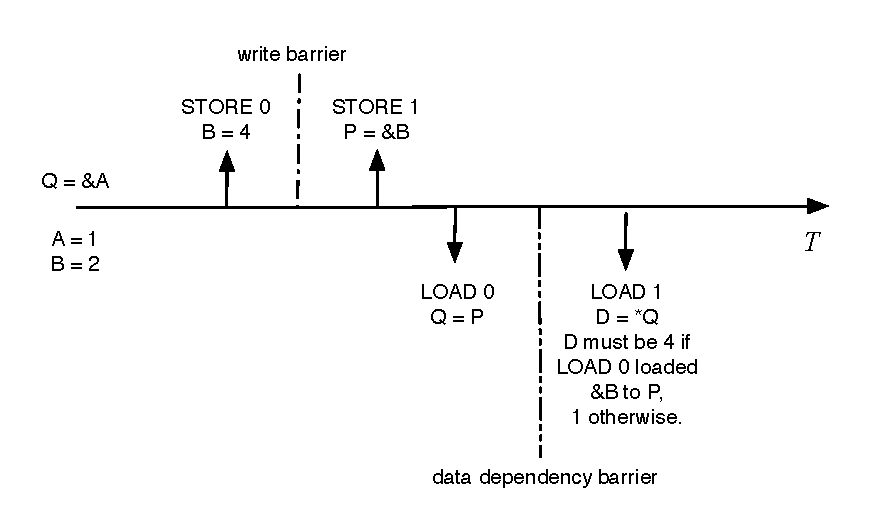
\includegraphics[scale=0.75]{fig/wmb_ddmb}
      \caption{写屏障及其配对的数据依赖屏障}
      \label{fig:ddmb}
    \end{figure}
    需要指出的是,
    如果没有那个data dependency barrier,
    在某些硬件体系结构(如:Alpha)上,
    完全可能发生Q = \&B但是D = 2这样的结果。
    导致这一看似违反因果律的一种可能原因是:
    P被读入奇数行的cache line而B被读入偶数行的cache line中,
    并且偶数行的cache line过于繁忙,
    于是P已经被更新但读取的B仍然是未被更新的cache值。
  \item {\em 读屏障}:
    读屏障保证了对系统的其它组件而言,
    屏障之前的读指令(LOAD)总是在在屏障之后的读指令之前被观察到。
    读屏障隐含了数据依赖屏障。
    同样地读屏障并不影响任何的写内存指令。
    通常写屏障之前的写入与读屏障或数据依赖屏障之后的读取相对应。
  \item {\em 通用屏障}:
    就是读写屏障,
    所有的读和写被屏障部分地有序化。
  \item {\em 半透屏障}:
    LOCK保证其后的访存操作不会出现在锁之前,
    同时UNLOCK保证之前的访存操作不会漏到其后,
    硬件必须保证这一半透屏障特性,
    否则同步就无从谈起了。
\end{itemize}

引起访存乱序还可能源自于编译器,
很多时候编译器会将它认为无依赖关系的指令重排实现优化,
如果希望某部分代码编译后指令一定要出现在另外一部分之前,
可以使用barrier()函数。

内存屏障一个重要场景是外设的MMIO实现。
外设的地址空间(端口,寄存器,内存)可以有两种方式访问,
一种称为{\em I/O Mapped},
另一种称为{\em Memory Mapped},
前一种方式使用\ins{in}/\ins{out}指令来访问外设地址空间,
后一种方式将外设地址空间映射到虚拟地址空间中,
一般建议用\ins{readb/w/l}或\ins{writeb/w/l}指令访问,
称为MMIO,
但是某些平台支持直接用指针访问I/O内存映射,
这种情况就必须适当使用内存屏障,
因为无论是CPU还是编译器都不知道外设地址空间到虚拟地址空间映射的逻辑。

\subsection{零拷贝}
假设一个简单场景,
用户进程调用read将数据读入一个用户态缓冲区,
而后将其通过write写入一个socket发送出去。
这个简单的应用实际上在内核空间导致了四次数据拷贝。
\begin{enumerate}
  \item DMA引擎将磁盘数据拷贝到内核缓冲区(假设数据不在page cache中)
  \item 接收到的数据被从内核缓冲区拷贝到read系统调用指定的用户态缓冲区中
  \item write系统调用把用户态缓冲区中数据拷贝到内核socket缓冲区
  \item 网卡的DMA引擎将内核的socket缓冲区中数据拷贝发送
\end{enumerate}
以上四个拷贝中的多数是可以通过某些硬件软件手段避免。

第一个可以想到的使用mmap替代read,
也就是将内核缓冲区映射到用户的虚拟地址空间中,
于是以上的第2个拷贝操作可以避免。
使用mmap的一个问题是,
当write过程中如果有另外一个进程把文件截断({\em truncate}),
写进程将收到一个SIGBUS信号。
显然在用户中代码简单地忽略SIGBUS信号绝对不可行,
一个正确的做法是在mmap之前先使用fcntl对该文件上一个租约({\em lease})锁,
当有其它进程试图截断该文件时,
本进程会收到一个RT\_SIGNAL\_LEASE信号,
其中RT代表real time。
进程的写操作被中断,
但是该写操作的errno为success,
返回已经写入的字节数。
而后进程被SIGBUS杀死。

自2.1版本起,
Linux内核提供sendfile系统调用,
其作用类似于上述mmap+write方案,
可以减少一次从内核缓冲区向用户态缓冲区的拷贝。
当有其它进程试图截断正在访问的文件时,
返回已处理的数据字节数并将errno设为成功,
不同的是,
系统仅发送RT\_SIGNAL\_LEASE而不发送SIGBUS。

需要更进一步提高效率,
从文件系统缓冲区向socket缓冲区的拷贝需要想办法消除。
这就需要硬件支持\emph{scatter/gather I/O}的功能,
如本例中,
如果网卡的发送缓冲区可以是分散的内存位置,
而且网卡可以通过一次DMA操作即可将这分散的数据整合起来发送,
那么自文件系统缓冲区向socket缓冲区的那一次拷贝可以消除。
从内核2.4开始,
socket缓冲区被修改以支持此硬件功能,
简而言之就是传给硬件(DMA引擎)的参数不再是传统的地址+长度,
而是一个包含多个(可以不连续)的缓冲区的向量({\em vector}),
从而实现真正的CPU/OS层面上的``零拷贝''。

\subsection{访问用户空间地址}
编写内核模块代码过程,
当需要访问用户空间地址时必须使用%
\verb|copy_from_user|、
\verb|copy_to_user|、
\verb|get_user|、
以及\verb|put_user|系列函数完成,
不允许直接使用指针。

理论上说内核代码可以直接通过指针来访问用户地址空间中内容,
实际上在Linux下这样做也偶尔行得通,
但更多时候会导致内核或应用程序崩溃。
这是Linux内核基于一些简单原则所做的设计决定,
并非因为有不可逾越的技术障碍。

{\color{red}
In theory it's possible to access to the user space address
directly via a user land pointer,
and occasionally it works,
but most of the time this triggers a kernel oops.
Practically we use a serial of functions for user land address access,
for example,
\verb|copy_from_user|,
\verb|copy_to_user|,
\verb|get_user|,
\verb|put_user|,
etc.}

首先一个原则是内核态一般不允许触发缺页异常,
除了以下两个特例,
包括:
\begin{itemize}
  \item 缺页地址落在内核\verb|vmalloc|区
  \item 缺页地址位于用户地址空间,
  并且引发异常的代码位于\verb|fixup|段中
\end{itemize}
其它情况将引发{\em kernel oops},
并且内核将发送\verb|SIGKILL|杀死用户进程。
细节详见\path{do_page_fault}函数。

\verb|fixup|文本段专门为了处理内核代码访问用户空间地址而设立。
所有需要访问用户空间的代码(大多是系统调用)使用统一的接口,
接口实现都放置({\em relocate})在\verb|fixup|文本段内,
称为{\em exception tables},
\verb|do_page_fault|调用\verb|search_exception_tables|搜索触发缺页的指令。

另外值得一提的是\verb|vmalloc|区的所有页映射已经建立,
为什么还可能触发缺页?
原因是\verb|vmalloc|区的映射建立的是一个内核主页表
(即所有进程的内核空间模板),
具体到某个进程,
映射可能并未建立,
所以这种异常发生之后,
内核调用\verb|vmalloc_fault|拷贝内核主页表给该进程。

\subsection{下划线函数名前缀}
历史上,
单下划线前缀被用于声明某些本应是内部私有,
但最终出于某些技术原因为外不可见的函数。
Linux应该也延续了这一传统。

Linux内核种有些函数以双下划线为前缀示意直接调用该函数要谨慎,
因为它们仅完成核心功能,
不执行参数校验、互斥等重要过程。
如果可能尽量使用不带双下划线的``安全''接口。

\subsection{常用宏定义}
\begin{itemize}
  \item {\tt offsetof}:取一个结构中某个域在该结构的偏移位置,
    当不能使用编译器提供的功能时,
    使用一个小技巧用宏实现:
    \inputclisting{src/offsetof.c}
                  {offsetof macro}{offsetof}
    %\lstinputlisting[language={C},%
    %                 caption={offsetof macro in C},%
    %                 label={lst:offsetof}]%
    %  {#define offsetof(TYPE, MEMBER) ((size\_t) \&((TYPE *)0)->MEMBER)}
  \item {\tt container\_of}:已知域的地址,求包含其域的结构地址:
    \inputclisting{src/container_of.c}
                  {container\_of macro}{cof}
  \item {\tt min(x, y)}:返回x和y中较小者,
    一个粗糙的宏定义如下,
    这个宏定义存在于无数的程序中,
    包括一些驱动程序,
    \inputclisting{src/wrong_min.c}
                  {naive min macro}{wmin}
    参数带着括号使用,
    这个宏定义依然是错的,
    原因在于该宏在程序执行时某个参数将被访问两次,
    于是象min(x++, y++)这样的调用将导致或者是x或者是y被自加两次。
    解决方法是使用gcc的\verb|({...})|扩展,
    在代码块内定义临时变量来存放参数,
    返回临时变量中较小的那一个:
    \inputclisting{src/min.c}
                  {correct min macro}{min}
    有意思的地方在于那个永不为真的地址比较,
    比较是为了在编译阶段就能察觉传入参数类型不一致,
    由于该比较对外界毫无影响,
    编译器将发出``has no effect''警告,
    加(void)的目的就是消除该警告,
    事实上该语句将不会被编译为任何指令。
    通常需要返回值的宏考虑使用\verb|{...}|扩展。
  \item {\tt do\{...\}while(0)},
    在Linux内核中多数包含多条语句的宏定义采用do\{...\}while(0)
    的形式,而不是简单地将多条语句包含在一对花括号中。
    首先考虑不采用包含在一对花括号中的情况,
    多条语句顺序在宏中出现,
    考虑如下代码
    \inputclisting{src/bad_macro0.c}
                  {bad macro0}{bm0}
    调用宏的语句出现在if/else场景中,
    宏展开后statement1;出现在else之前,
    导致C语法错误。
    将多条语句包含在一对花括号中可以解决问题,
    但是调用宏的语句不能以分号结束,
    如下代码正确但是有点丑陋,
    C语句不以分号结束不符合普遍编程习惯:
    \inputclisting{src/bad_macro1.c}
                  {bad macro1}{bm1}
    解决方法就是内核所使用的do\{...\}while(0)小技巧:
    \inputclisting{src/good_macro.c}
                  {good macro}{gm}
\end{itemize}

\subsection{Buddy System}
无控制的任意尺寸页帧分配和释放最终将%
导致内存中布满了分隔的大量小尺寸可用页帧,
从数量上虽然有足够可用内存,
却没有一块连续的大尺寸页帧满足分配请求,
这就是所谓外部碎片。
{\em Buddy System}设计用于有效减少外部碎片。

Linux下Buddy System的思路如下:
\begin{enumerate}
  \item 将所有页帧归为不同的组,
    每个组包含连续也帧数是2的$n$幂,
    指数$n$取值自0至10,
    相同指数的页帧用链表组织,
    11个链表头保存在zone的mem\_map数组域中,
    指数即作为该数组的索引。
  \item 当试图分配尺寸为2的m次幂个页帧时,
    首先查找指数为m的组,
    如果有可用页帧组则返回该组,
    否则查找指数加一的组,
    关键的是,
    当实际分配的页帧组指数小于从中分配的页帧组指数是,
    该页帧组剩余的页帧组要被相应插入到指数小的链表中;
  \item 释放一组页帧时,
    如果该组有一个“伙伴”,
    则和其伙伴合并为一个指数高一级的组
    继续找伙伴合并过程直至无法找到合适的伙伴。
    两个页帧组可以成为伙伴必须满足:
    \begin{enumerate}
      \item 两个组相邻
      \item 两个组有相同的尺寸,假设为$b$
      \item 两个组如果合并为一个大组,
        大组的第一个页的起始地址必须为$2 \times b \times 2^{12}$的整数倍,
        换句话说就是合并后的大组首地址按$2b$页方式对齐,
        要找一个组和其伙伴合并后的大组的首地址用异或实现:
        $buddy\_idx = page\_idx \XOR (1 <\!<\! b)$,
        异或实际效果是switch了一个地址的第$b$位,
        亦即如果该位原来为0,
        结果是比该组地址高$b \times 2^{12}$的地址,
        否则是比该组地址低$b \times 2^{12}$的地址,
        这就保证了合并后的大组首地址按$2b$页对齐
    \end{enumerate}

\end{enumerate}

\subsection{Slab Allocator}
\begin{figure}[!ht]
\centering
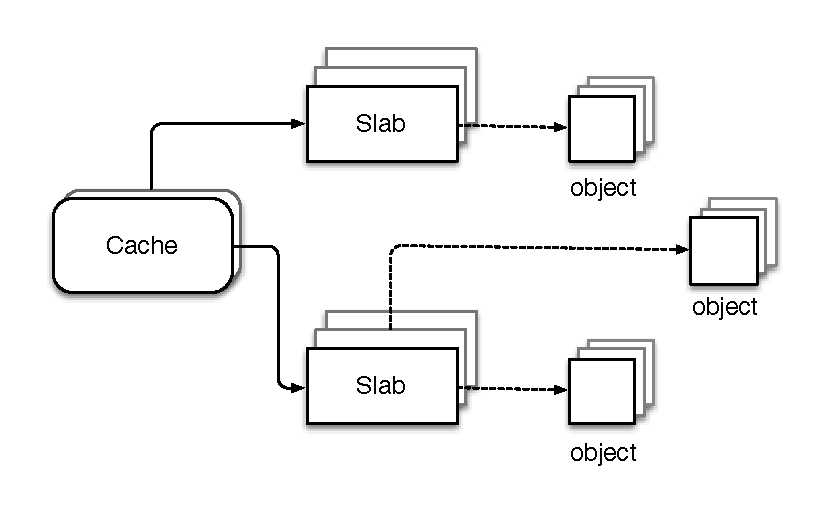
\includegraphics[scale=0.8]{fig/slab}
\caption{Cache、Slab,及对象}
\label{fig:slab}
\end{figure}

{\em Slab Allocator}解决如下问题:
\begin{itemize}
  \item 统一管理所谓{\em free list}缓存,
    对于频繁分配释放的数据结构,
    一般程序员会一次性分配大块内存用作缓存,
    即数据结构从缓存中分配,
    释放数据结构也不立即交还系统(譬如Buddy System)而是放入free list中%
    以备随时再次分配。
    这种free list方案带来的问题是,
    内核无法统一管理,
    于是干脆提供一个为所有模块服务的缓存机制。

  \item 内部碎片,
    由于内核分配以页为单位,
    如果不有效管理利用,
    一个页内会有无用空间,积少成多数量也很可观,
    这就是所谓内部碎片问题。

  \item 内核的开发人员可以在slab这一层加入一些高级的优化策略,
    譬如,上色降低相同类型的缓存被放置于同一条缓存线上({\em cache line})。
\end{itemize}

如图\,\ref{fig:slab}\,所示:
一个数据结构占据一段连续的内存,
称为一个“对象”,
用于存放一组相同数据类型的对象称为“slab”,
一个slab可以占据一个或多个连续的物理页帧,
所有的slab组成该类型的“cache”。

如图\,\ref{fig:slabc}\,所示,
颜色属性尽量将一个slab和另一个同类型slab对象的起始地址错开,
降低它们落入同一条缓存线的几率。

\begin{figure}[!ht]
\centering
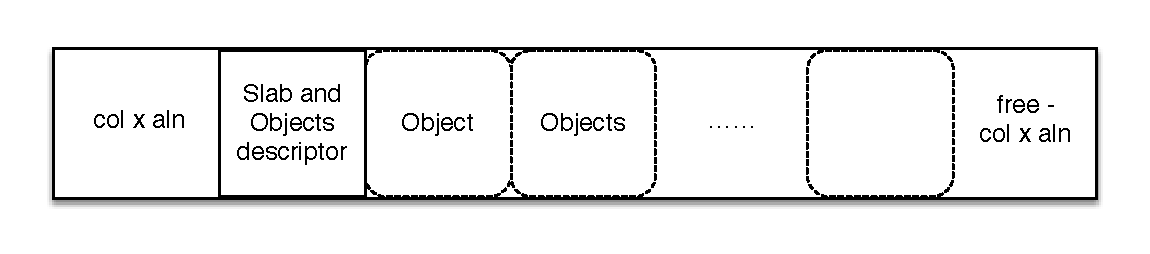
\includegraphics[scale=0.72]{fig/slab_color}
\caption{Slab Coloring}
\label{fig:slabc}
\end{figure}
